{\color{solution}

\begin{enumerate}
	\item
	\begin{itemize}
		\item[``$\Rightarrow$'']Let $Q$ be isometric, i.e., $\|Q x\|_2=\|x\|_2$ for all $x \in \Rn$. (\underline{to show}: $Q^\top Q = I$ or equivalently $(Q^\top Q)_{ij} = \delta_{ij}$, where $\delta_{ij}$ denotes the Kronecker delta) Following the hint we first observe that 
				\begin{align*}
		(Q^\top Q)_{ij} 
		= (e_i,Q^\top Q e_j)_2= (Qe_i, Q e_j)_2.
		\end{align*}
		 Second, by polarization formula and the isometry property we obtain
		\begin{align*}
		 (Q x,Q y)_2
		 &= \frac{1}{4} \left(\|Q x+Q y\|^2-\|Q x-Q y\|^2\right)\\
		 &=\frac{1}{4} \left(\|Q (x+y)\|^2-\|Q (x-y)\|^2\right)\\
		 &=\frac{1}{4} \left(\|x+y\|^2-\| x-y\|^2\right)
		\end{align*}
		for all $x,y\in\mathbb{R}^n$. Now we insert the standard basis vectors $x=e_i, y=e_j$ and obtain
		\begin{align*}
		  (Q^\top Q)_{ij} 
		  &= (Q e_i,Q e_j)_2\\
		  &=\frac{1}{4} \left(\|e_i+e_j\|^2-\| e_i-e_j\|^2\right)\\
		  &=\delta_{ij},
		 \end{align*}
		where $\delta_{ij}$ denotes the Kronecker delta. Thus, $Q$ is orthogonal.
		\item[``$\Leftarrow$''] Let $Q$ be orthogonal, i.e., $Q ^\top Q = I$. Then $\|Q x\|_2=\sqrt{x^\top Q ^\top Q  x}=\|x\|_2$. 
	\end{itemize} 	
	\item  
	\begin{enumerate}
		\item By computing the matrix-matrix product we find	$$Q_\alpha^TQ_\alpha = 
		\begin{pmatrix}
		\sin^2\alpha + \cos^2\alpha  & - \cos \alpha\sin \alpha + \sin \alpha \cos \alpha \\
		- \sin \alpha\cos \alpha + \cos \alpha\sin \alpha  &\sin^2\alpha + \cos^2\alpha \\
		\end{pmatrix} = I .
		$$
		\item First note that $$Q_{\pi/4} = \begin{pmatrix}
		\cos \pi/4 & -\sin \pi/4\\
		\sin \pi/4 & \cos \pi/4\\
		\end{pmatrix} = \frac{1}{\sqrt{2}}\begin{pmatrix}
		1& - 1\\
		1 &  1 \\
		\end{pmatrix}.$$
		 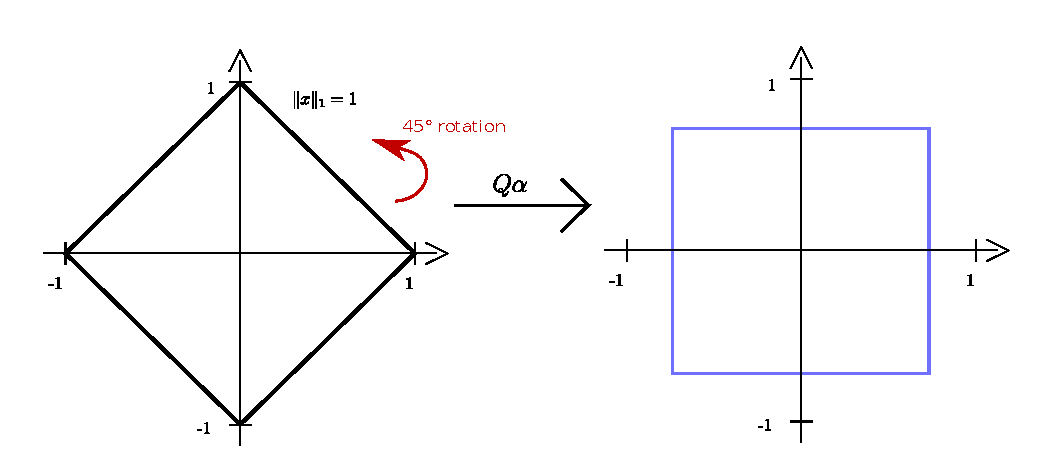
\includegraphics[width=0.8\textwidth]{orthogonalisometricmatrix.pdf}\\
		 \textit{Remark:} We have rotated the unit $\|\cdot\|_1$-norm ball to a $\|\cdot\|_\infty$-norm ball of radius $\frac{1}{\sqrt{2}}$.
		 
	\end{enumerate}
	
\end{enumerate}	

	
	
	
}

